% Вторая глава курсовой работы: обучение и оценка моделей машинного обучения
%
\chapter{\MakeUppercase{Машинное обучение на больших данных}}\label{ch:second}


\vspace{\baselineskip}
Во второй главе рассматривается применение средств машинного обучения Apache Spark MLlib к подготовленному набору US Accidents. В соответствии с постановкой лабораторной работы № 2 решаются две задачи: прогнозирование длительности дорожно-транспортного происшествия с помощью линейной регрессии и бинарная классификация происшествий по признаку тяжести с помощью случайного леса. Для обеих задач подготовка признаков, обучение и оценка моделей организованы в виде воспроизводимых конвейеров \texttt{Pipeline}, предусмотренных API Spark MLlib для построения последовательностей преобразований и алгоритмов машинного обучения \cite{spark352mllib, spark352pyspark}.

\vspace{\baselineskip}
\section{Задача регрессии}

\subsection{Постановка задачи регрессии}\vspace{\baselineskip}

Первая задача машинного обучения состоит в прогнозировании длительности дорожно-транспортного происшествия. В качестве целевой переменной используется \texttt{Duration\_min} -- продолжительность происшествия в минутах, вычисленная как разность между временем его окончания и временем начала. На этапе подготовки данных верхняя граница длительности была ограничена значением 2880 мин, поэтому целевая переменная не содержит экстремальных значений, соответствующих многолетним интервалам.

Требуется построить модель линейной регрессии, которая по характеристикам происшествия, погодным условиям, инфраструктуре и временным признакам оценивает значение \texttt{Duration\_min}. В качестве алгоритма выбран \texttt{LinearRegression} из библиотеки Spark MLlib; данный метод относится к базовым алгоритмам регрессионного анализа и широко рассматривается в учебных материалах по машинному обучению \cite{spark352mllib, yandex2024ml}. Данный алгоритм позволяет оценить линейную зависимость целевого признака от набора предикторов и получить интерпретируемые коэффициенты модели.

Выбор целевой переменной обусловлен результатами разведочного анализа, выполненного в первой главе. Длительность является количественной характеристикой результата происшествия, не содержит пропусков и может быть рассчитана из временных меток. Вместе с тем линейная связь длительности с отдельными числовыми признаками оказалась слабой: наибольшая по модулю корреляция наблюдалась с \texttt{Distance(mi)} и составляла 0,122. Поэтому заранее ожидалось, что линейная модель будет иметь ограниченную предсказательную способность.

Качество модели оценивается по следующим метрикам:
\begin{itemize}
    \item среднеквадратичная ошибка (RMSE), характеризующая типичный масштаб ошибки с повышенным весом крупных отклонений;
    \item коэффициент детерминации ($R^2$), показывающий долю вариации целевой переменной, объясняемую моделью;
    \item средняя абсолютная ошибка (MAE), характеризующая среднее абсолютное отклонение предсказаний от фактических значений.
\end{itemize}

Для проверки полезности модели результаты дополнительно сравниваются с базовым предсказателем (baseline), который для всех объектов возвращает медиану целевой переменной обучающей выборки. Такое сравнение позволяет определить, извлекает ли линейная модель закономерности из признаков или её качество близко к константному прогнозу.

\vspace{\baselineskip}\subsection{Подготовка признаков и обучение модели}\vspace{\baselineskip}

Обучение выполнялось на очищенной таблице Apache Iceberg \texttt{otpushchennikov\_us\_accidents\_processed}, содержащей 7\,728\,394 записи и 38 полей. Обработка производилась средствами Apache Spark 3.5.2 на кластере Apache Hadoop с использованием YARN. Для запуска Spark-сессии использовался режим \texttt{client}; выделялись два исполнителя по 8 ядер и 12 ГБ оперативной памяти каждый, а для драйвера -- 2 ядра и 4 ГБ памяти.

Перед формированием вектора признаков были исключены поля, не предназначенные для непосредственного обучения. Идентификатор \texttt{ID} уникален для каждой строки и не несёт обобщаемой информации. Временные метки \texttt{Start\_Time} и \texttt{End\_Time} не включались, поскольку из них уже были получены признаки месяца, дня недели и часа, а разность между ними используется для вычисления целевой переменной. Координаты начала происшествия исключались, поскольку для описания местоположения использовался штат. Также были исключены \texttt{City}, \texttt{County}, \texttt{Zipcode}, \texttt{Timezone} и \texttt{Airport\_Code}: высокая кардинальность этих категориальных признаков привела бы к чрезмерному увеличению размерности после кодирования. Признак \texttt{Severity} не использовался, так как он является целевой переменной второй задачи и не должен выступать предиктором длительности в рассматриваемой постановке.

Для подготовки оставшихся признаков применялись следующие преобразования:
\begin{itemize}
    \item категориальные признаки с ограниченным числом значений преобразовывались с помощью \texttt{StringIndexer} и \texttt{OneHotEncoder}. Такое кодирование не задаёт искусственного порядка между категориями;
    \item количественные признаки нормализовались с помощью \texttt{MinMaxScaler}. Приведение признаков к сопоставимому масштабу необходимо для корректной работы регуляризации линейной модели;
    \item логические признаки преобразовывались в числовые значения 0 и 1;
    \item признак \texttt{Precipitation(in)} бинаризовался по порогу 0,1 дюйма, поскольку после заполнения пропусков нулём его распределение было сосредоточено преимущественно в нуле.
\end{itemize}

Все этапы преобразования признаков и сама модель объединялись в единый конвейер \texttt{Pipeline}. Это важно для корректной кросс-валидации: параметры индексаторов и масштабирования вычисляются на обучающей части каждого фолда, а затем применяются к соответствующей проверочной части. Таким образом, информация из проверочных данных не используется при обучении преобразований.

Основные этапы конвейера регрессии показаны в коде ниже. Сначала категориальные значения индексируются и кодируются методом one-hot, затем количественные признаки объединяются и масштабируются, после чего формируется общий вектор признаков для линейной регрессии.

\begin{code}
string_indexer = StringIndexer(
    inputCols=categorical_features,
    outputCols=indexed_categorical_features,
    handleInvalid="keep")
onehot_encoder = OneHotEncoder(
    inputCols=indexed_categorical_features,
    outputCols=onehot_categorical_features,
    dropLast=True, handleInvalid="keep")
numeric_scaler = MinMaxScaler(
    inputCol="numeric_vector",
    outputCol="numeric_vector_scaled")
linear_regression = LinearRegression(
    featuresCol="features", labelCol=label_col,
    standardization=False, maxIter=max_iter)
pipeline = Pipeline(stages=[
    string_indexer, onehot_encoder, vector_num_assembler,
    numeric_scaler, binarizer, vector_all_assembler,
    linear_regression])
\end{code}

После объединения этапов конвейер обучается как единый объект. Это позволяет применять одинаковую последовательность преобразований как к обучающим, так и к тестовым данным и исключает раздельное ручное выполнение операций.

Исходный набор случайным образом разделялся на обучающую и тестовую части в соотношении 80/20. Для выбора параметров модели применялась пятиблочная кросс-валидация. Подбирались два параметра линейной регрессии: \texttt{regParam}, определяющий силу регуляризации, и \texttt{elasticNetParam}, задающий соотношение $L_1$- и $L_2$-регуляризации. Всего проверялось девять комбинаций параметров. В качестве критерия выбора использовалась минимальная RMSE на кросс-валидации.

Перед полным подбором параметров было измерено время одного обучения конвейера на полной обучающей выборке: 108,8 с. Для девяти комбинаций и пяти фолдов требовалось выполнить 45 обучений, поэтому предварительная оценка продолжительности подбора составляла около 81,6 мин. Фактический подбор занял приблизительно 56 мин: после первого прогона обучающая выборка находилась в кеше Spark, что сократило время последующих обучений.

Для выбора параметров использовалась пятиблочная кросс-валидация. Фрагмент настройки кросс-валидации приведён в коде ниже. В качестве оценщика применялась RMSE, а сравнение выполнялось на одинаковых разбиениях данных.

\begin{code}
cross_validator = CrossValidator(
    estimator=pipeline,
    estimatorParamMaps=param_grid,
    evaluator=cv_evaluator,
    numFolds=5)
\end{code}

Пятиблочная схема обеспечивает сравнение комбинаций параметров на нескольких разбиениях обучающей выборки. В качестве итоговой выбирается комбинация с наименьшей средней ошибкой RMSE.


\vspace{\baselineskip}\subsection{Анализ полученных результатов}\vspace{\baselineskip}

Минимальная ошибка кросс-валидации была получена при \texttt{regParam = 0,01} и \texttt{elasticNetParam = 0,0}. Последнее значение соответствует чистой $L_2$-регуляризации. Результаты отдельных комбинаций параметров приведены в таблице~\ref{tab:lr-cv}.

\begin{table}[H]
    \centering
    \caption{Результаты подбора параметров линейной регрессии}
    \label{tab:lr-cv}
    \small
    \begin{tabular}{|c|c|c|}
        \hline
        \centering\arraybackslash \texttt{regParam} & \centering\arraybackslash \texttt{elasticNetParam} & \centering\arraybackslash RMSE на кросс-валидации \\
        \hline
        0,01 & 0,0 & 178,2996 \\
        \hline
        0,01 & 0,5 & 178,3007 \\
        \hline
        0,01 & 1,0 & 178,3052 \\
        \hline
        0,10 & 0,0 & 178,4885 \\
        \hline
        1,00 & 1,0 & 180,6160 \\
        \hline
    \end{tabular}
\end{table}

Разница между первыми тремя комбинациями невелика, однако увеличение силы регуляризации приводит к ухудшению результата. Это согласуется с большим размером обучающей выборки: на этапе обучения использовалось 6\,180\,705 строк при 123 признаках. Количество наблюдений значительно превышает число параметров, поэтому сильное ограничение коэффициентов не требуется. В лучшей модели наибольший по модулю коэффициент составил 647,75, свободный член -- 159,90. Четыре коэффициента оказались равны нулю вследствие вырожденных столбцов после масштабирования.

На тестовой выборке, включавшей 1\,546\,700 записей, были получены значения метрик, представленные в таблице~\ref{tab:lr-test}.

\begin{table}[H]
    \centering
    \caption{Качество линейной регрессии на тестовой выборке}
    \label{tab:lr-test}
    \small
    \begin{tabular}{|l|r|}
        \hline
        \centering\arraybackslash Метрика & \centering\arraybackslash Значение \\
        \hline
        RMSE модели & 178,54 мин \\
        \hline
        $R^2$ модели & 0,0472 \\
        \hline
        MAE модели & 85,00 мин \\
        \hline
        Медиана целевой переменной в обучающей выборке & 74,85 мин \\
        \hline
        RMSE базового предсказателя & 187,65 мин \\
        \hline
        Улучшение относительно baseline & 4,85\,\% \\
        \hline
    \end{tabular}
\end{table}

Значение RMSE на тестовой выборке близко к результату кросс-валидации, что говорит об отсутствии заметного расхождения между проверочными фолдами и тестовой выборкой. При этом коэффициент детерминации равен всего 0,0472. Следовательно, линейная модель объясняет менее пяти процентов вариации длительности происшествий. По сравнению с базовым предсказателем ошибка уменьшилась на 4,85\,\%, то есть выигрыш оказался небольшим.

Для дополнительной проверки процесса оптимизации в ноутбуке построен график изменения функции ошибки при обучении методом L-BFGS. Результат визуального контроля и метрики на обучающей выборке представлены на рисунке~\ref{fig:lr-training}.

\begin{figure}[H]
    \centering
    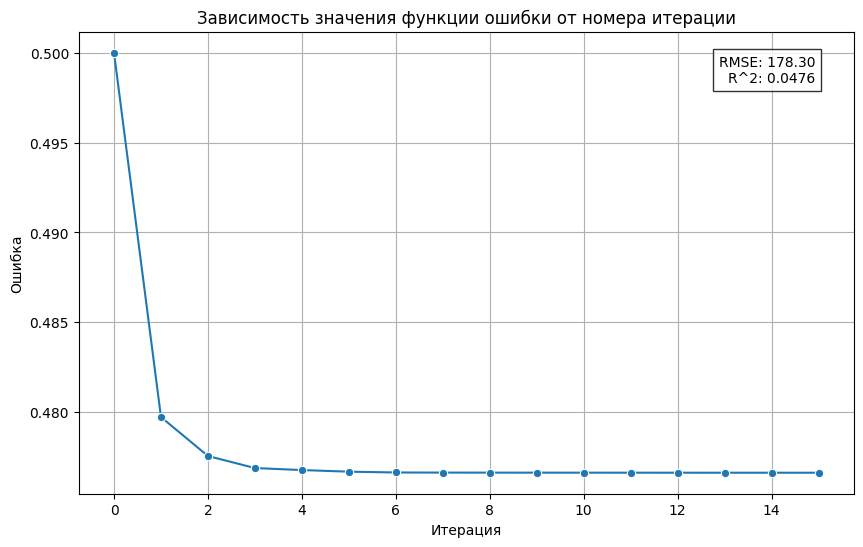
\includegraphics[width=0.88\textwidth]{Content/Images/lab2_regression_diagnostics.png}
    \caption{Диагностика процесса обучения модели линейной регрессии}
    \label{fig:lr-training}
\end{figure}

Дополнительный анализ ошибок по децилям фактической длительности показал выраженное стремление модели к среднему значению. Средние предсказания модели располагались в узком диапазоне от 100 до 137 мин, тогда как средние фактические значения по децилям изменялись от 25,7 до 481,1 мин. В результате короткие происшествия модель существенно переоценивает, а длительные -- недооценивает. Это типичное поведение линейной регрессии при слабой связи признаков с целевой переменной и асимметричном распределении длительности.

Таким образом, построенная линейная модель формально решает задачу регрессии, однако её практическая предсказательная способность ограничена. Полученный результат не означает, что обработка данных или распределённое обучение выполнены некорректно: скорее, доступные признаки недостаточно хорошо описывают длительность происшествия в рамках линейной зависимости. Для повышения качества в дальнейшем можно исследовать нелинейные алгоритмы или преобразование целевой переменной, например логарифмирование.

\vspace{\baselineskip}
\section{Задача бинарной классификации}

\subsection{Постановка задачи бинарной классификации}\vspace{\baselineskip}

Вторая задача состоит в определении того, относится ли дорожно-транспортное происшествие к категории тяжёлых. Исходный признак \texttt{Severity} принимает значения от 1 до 4 и представляет собой упорядоченную шкалу тяжести. Для решения задачи бинарной классификации он преобразуется в целевую переменную \texttt{is\_severe} по правилу:
\begin{equation}
    \label{eq:is-severe}
    \text{is\_severe} =
    \begin{cases}
        1, & \text{если } \text{Severity} \geq 3,\\
        0, & \text{если } \text{Severity} < 3.
    \end{cases}
\end{equation}

Таким образом, положительный класс объединяет происшествия третьего и четвёртого уровней тяжести, а отрицательный -- первого и второго. Выбор порога 3 обусловлен смыслом исходной шкалы и распределением данных: тяжёлые классы составляют меньшую часть набора, поэтому задача одновременно позволяет исследовать обучение классификатора на несбалансированных данных.

Формирование бинарной метки выполнялось непосредственно средствами PySpark. Преобразование исходного признака \texttt{Severity} в целевую переменную \texttt{is\_severe} показано в коде ниже.

\begin{code}
label_col = "is_severe"
df = df.withColumn(
    label_col,
    when(col("Severity") >= 3, 1)
    .otherwise(0).cast(IntegerType()))
\end{code}

В результате происшествия с уровнями тяжести 3 и 4 получают метку 1, а происшествия уровней 1 и 2 — метку 0. Полученная переменная используется как целевой признак классификатора.

В качестве алгоритма выбран \texttt{RandomForestClassifier} -- ансамбль решающих деревьев. Случайный лес строит множество деревьев на случайных подвыборках наблюдений и признаков, а затем агрегирует их предсказания. Этот принцип ансамблирования подробно описан в классической работе Л. Бреймана о случайных лесах и реализован в Spark MLlib \cite{breiman2001random, spark352mllib}. В отличие от линейной модели, деревья способны учитывать нелинейные зависимости и взаимодействия между признаками. Это соответствует результатам первой главы, где линейные корреляции отдельных числовых признаков с тяжестью происшествия были невелики.

Качество классификации оценивается с помощью следующих метрик, широко используемых при решении задач бинарной классификации \cite{yandex2024ml, spark352mllib}:
\begin{itemize}
    \item точность (Precision) -- доля действительно тяжёлых происшествий среди объектов, отнесённых моделью к положительному классу;
    \item полнота (Recall) -- доля найденных моделью тяжёлых происшествий среди всех фактически тяжёлых происшествий;
    \item F1-мера -- гармоническое среднее точности и полноты;
    \item площадь под ROC-кривой (AUC ROC) -- характеристика способности модели ранжировать положительные объекты выше отрицательных.
\end{itemize}

Для рассматриваемой задачи особенно важно не пропустить тяжёлое происшествие. Поэтому дополнительно ставится условие: подобрать порог вероятности положительного класса так, чтобы полнота была не ниже 60\,\%, и при этом получить максимально возможную точность при данном ограничении.

\vspace{\baselineskip}\subsection{Подготовка признаков и обучение модели}\vspace{\baselineskip}

Для классификации использовалась та же очищенная таблица Apache Iceberg, содержащая 7\,728\,394 записи. Признаки, не предназначенные для обучения, исключались по тем же причинам, что и в задаче регрессии: уникальный идентификатор, исходные временные метки, координаты и категориальные поля с высокой кардинальностью. В отличие от регрессионной задачи, \texttt{Duration\_min} сохранялся в наборе признаков, поскольку в этой постановке он связан с тяжестью происшествия. При этом такое решение следует рассматривать как ограничение прикладной интерпретации: длительность известна после завершения происшествия и не может использоваться в модели раннего предупреждения без утечки информации о результате.

Подготовка признаков отличалась от конвейера регрессии. Категориальные признаки преобразовывались с помощью \texttt{StringIndexer} без one-hot-кодирования. Для деревьев решений достаточно числовых индексов категорий, а создание большого числа бинарных столбцов увеличило бы размерность вектора. Количественные признаки не масштабировались, поскольку разбиения деревьев по порогам значений не зависят от монотонного изменения масштаба. Бинарные признаки приводились к значениям 0 и 1. Признак осадков, как и в задаче регрессии, преобразовывался в бинарный по порогу 0,1 дюйма.

После подготовки признаков формировался конвейер \texttt{Pipeline}, включавший индексирование категорий и случайный лес. Параметр \texttt{handleInvalid = keep} обеспечивал обработку неожиданных категориальных значений, которые могли встретиться при применении конвейера. Для категориальных признаков использовался параметр \texttt{maxBins = 64}. Это значение необходимо, поскольку признак \texttt{State} содержит 52 категории, а значение по умолчанию 32 недостаточно для построения дерева с таким категориальным предиктором.

Фрагмент построения модели приведён в коде ниже. В эксперименте использовались 50 деревьев, 64 корзины для категориальных признаков и фиксированное начальное значение генератора случайных чисел 2026, обеспечивающее воспроизводимость.

\begin{code}
random_forest = RandomForestClassifier(
    featuresCol="features",
    labelCol=label_col,
    predictionCol="prediction",
    numTrees=50,
    maxBins=64,
    seed=2026)
pipeline = Pipeline(stages=[
    string_indexer, binarizer,
    vector_all_assembler, random_forest])
\end{code}

После формирования конвейера случайный лес обучается на подготовленном векторе признаков. Параметр глубины дерева дополнительно выбирался на этапе кросс-валидации, а фиксированное начальное значение генератора случайных чисел делает эксперимент воспроизводимым.

Распределение целевого признака было несбалансированным. Положительный класс \texttt{is\_severe = 1} включал 1\,504\,047 записей (19,47\,\%), отрицательный -- 6\,224\,347 записей (80,53\,\%). Если обучать классификатор непосредственно на таком распределении, модель может отдавать предпочтение большинству. Поэтому данные сначала разделялись на обучающую и тестовую выборки в отношении 80/20 со стратификацией по целевому классу. Стратификация сохраняет близкие доли классов в обеих частях.

Для балансировки обучающей выборки применялся oversampling: каждая запись положительного класса включалась в обучающую выборку в четырёх экземплярах. После этой операции обучающая часть содержала 4\,812\,684 отрицательных и 4\,980\,037 положительных записей, то есть классы стали практически сбалансированными. Тестовая выборка при этом не балансировалась и сохраняла исходное соотношение классов. Это принципиально важно: итоговые метрики должны отражать работу модели на естественном распределении данных, а не на искусственно сбалансированной выборке.

Для подбора гиперпараметров использовалась пятиблочная кросс-валидация. В качестве критерия выбора применялась AUC ROC. Основными параметрами случайного леса являлись \texttt{maxDepth} -- максимальная глубина дерева -- и \texttt{numTrees} -- количество деревьев в ансамбле. Предварительный замер показал, что обучение одного конвейера на полной сбалансированной выборке занимает около 285 с. Полная сетка из девяти комбинаций и пяти фолдов потребовала бы приблизительно 3,6 ч. Поэтому фактически была использована сокращённая сетка: значения глубины 4 и 6 при 50 деревьях, всего десять обучений с учётом пяти фолдов и итогового обучения.

\vspace{\baselineskip}\subsection{Анализ полученных результатов}\vspace{\baselineskip}

Результаты кросс-валидации представлены в таблице~\ref{tab:rf-cv}. Лучшей оказалась модель с глубиной дерева 6 и 50 деревьями в ансамбле.

\begin{table}[H]
    \centering
    \caption{Результаты подбора параметров случайного леса}
    \label{tab:rf-cv}
    \small
    \begin{tabular}{|c|c|c|}
        \hline
        \centering\arraybackslash \texttt{maxDepth} & \centering\arraybackslash \texttt{numTrees} & \centering\arraybackslash AUC ROC на кросс-валидации \\
        \hline
        6 & 50 & 0,7976 \\
        \hline
        4 & 50 & 0,7799 \\
        \hline
    \end{tabular}
\end{table}

Увеличение глубины дерева с 4 до 6 повысило AUC ROC с 0,7799 до 0,7976, то есть примерно на 1,8 процентного пункта. Это указывает на то, что более глубокие деревья лучше выявляют зависимости в данных. При этом размер сетки был ограничен по вычислительным соображениям: предварительный замер позволил оценить стоимость полного подбора до его запуска.

После выбора параметров модель была оценена на тестовой выборке из 1\,545\,186 записей. Сначала использовался стандартный порог классификации 0,5. Затем порог изменялся с учётом требования к полноте не менее 60\,\%. Основные результаты приведены в таблице~\ref{tab:rf-test}.

\begin{table}[H]
    \centering
    \caption{Метрики случайного леса на тестовой выборке}
    \label{tab:rf-test}
    \small
    \begin{tabular}{|l|c|c|c|}
        \hline
        \centering\arraybackslash Порог вероятности & \centering\arraybackslash Precision & \centering\arraybackslash Recall & \centering\arraybackslash F1 \\
        \hline
        0,50 & 0,3867 & 0,7767 & 0,5163 \\
        \hline
        0,61 & 0,4332 & 0,6018 & 0,5038 \\
        \hline
        \multicolumn{4}{|c|}{AUC ROC на тестовой выборке: 0,7970} \\
        \hline
    \end{tabular}
\end{table}

Значение AUC ROC на тестовой выборке составило 0,7970 и практически совпало с результатом кросс-валидации 0,7976. Это говорит о том, что оценка качества ранжирования устойчива к выбранному разбиению и не демонстрирует заметного ухудшения на отложенных данных.

На рисунке~\ref{fig:rf-curves} приведены ROC- и PR-кривые, построенные по вероятностям, рассчитанным моделью на тестовой выборке. Для удобства визуализации точки были агрегированы в 1000 интервалов по вероятности положительного класса. ROC-кривая характеризует соотношение полноты и доли ложноположительных срабатываний, а PR-кривая позволяет отдельно оценить точность при различных значениях полноты.

\begin{figure}[H]
    \centering
    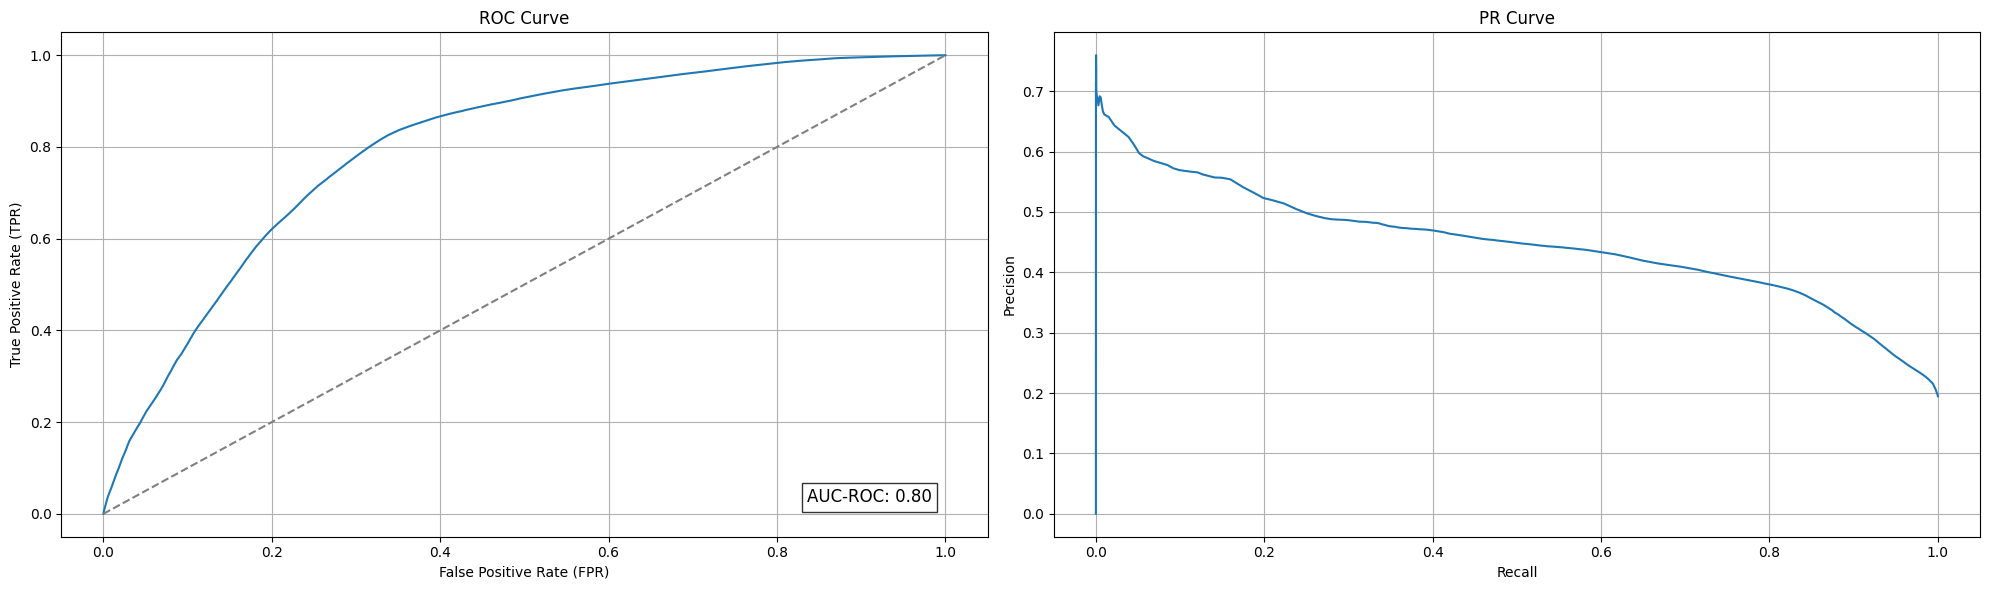
\includegraphics[width=0.95\textwidth]{Content/Images/lab2_classification_curves.png}
    \caption{ROC- и PR-кривые модели случайного леса на тестовой выборке}
    \label{fig:rf-curves}
\end{figure}

При стандартном пороге 0,5 полнота составила 0,7767: модель обнаруживает около 77,7\,\% тяжёлых происшествий. Однако точность равна только 0,3867, то есть значительная доля предсказаний положительного класса является ложноположительной. Такое соотношение объясняется в том числе балансировкой обучения: модель обучалась на почти равных долях классов, но проверялась на исходном распределении, в котором положительный класс составляет менее одной пятой всех записей.

Для выполнения условия $Recall \geq 0,60$ был подобран порог 0,61. При его использовании точность увеличилась до 0,4332, а полнота составила 0,6018. Таким образом, условие задачи выполняется, а доля правильных положительных предсказаний среди всех срабатываний возрастает. При этом F1-мера немного снижается -- с 0,5163 до 0,5038. Это ожидаемый компромисс: увеличение порога делает классификатор более избирательным, но приводит к пропуску большего числа тяжёлых происшествий. Выбор порога выполнялся по рассчитанной таблице вероятностей: выбиралось максимальное значение порога, при котором полнота не опускалась ниже 0,60. Соответствующий фрагмент выбора порога представлен в коде ниже.

\begin{code}
threshold_probability = pd_dataframe[
    pd_dataframe['TPR'] >= 0.60
]['probability'].max()
cv_model.bestModel.stages[-1].setThresholds([
    1 - threshold_probability,
    threshold_probability])
\end{code}

Полученное значение порога используется при преобразовании вероятностей в итоговые классы. Такой выбор позволяет выполнить требование к полноте, одновременно повышая точность по сравнению со стандартным порогом 0,5.

Для интерпретации результатов также важно учитывать несбалансированность тестовой выборки. Простой классификатор, всегда выбирающий отрицательный класс, достигает accuracy 0,8053 за счёт преобладания этого класса, но не обнаруживает ни одного тяжёлого происшествия. Поэтому accuracy не может выступать основной метрикой качества в данной задаче. Аналогично классификатор, всегда выбирающий положительный класс, имеет precision 0,1947, что соответствует доле положительного класса в тестовой выборке. Метрики Precision, Recall, F1 и AUC ROC дают более содержательную оценку работы модели.

Дополнительный анализ важности признаков показал, что наибольший вклад в предсказания вносят \texttt{Distance(mi)} (0,3047) и \texttt{Duration\_min} (0,2557). Далее следуют \texttt{Traffic\_Signal} (0,1024), \texttt{Weather\_Condition} (0,0851) и \texttt{Crossing} (0,0759). Суммарная важность пяти наиболее значимых признаков составляет 0,8238. Следовательно, модель в значительной степени опирается на сведения о протяжённости и длительности происшествия, а также на инфраструктурные и погодные характеристики.

Для сопоставления вкладов пяти наиболее значимых признаков их значения представлены на рисунке~\ref{fig:rf-feature-importance}. Длина каждой полосы пропорциональна рассчитанной моделью важности. Два первых признака заметно опережают остальные: суммарно на \texttt{Distance(mi)} и \texttt{Duration\_min} приходится около 56,0\,\% общей важности. Следующие три признака имеют существенно меньшие индивидуальные значения, хотя вместе также формируют значимую часть предсказательной структуры модели.

\begin{figure}[H]
    \centering
    \begin{tabular}{p{0.30\textwidth}p{0.53\textwidth}r}
        \texttt{Distance(mi)} & \rule{0.3047\textwidth}{0.45em} & 0,3047 \\
        \texttt{Duration\_min} & \rule{0.2557\textwidth}{0.45em} & 0,2557 \\
        \texttt{Traffic\_Signal} & \rule{0.1024\textwidth}{0.45em} & 0,1024 \\
        \texttt{Weather\_Condition} & \rule{0.0851\textwidth}{0.45em} & 0,0851 \\
        \texttt{Crossing} & \rule{0.0759\textwidth}{0.45em} & 0,0759
    \end{tabular}
    \caption{Пять наиболее значимых признаков модели случайного леса}
    \label{fig:rf-feature-importance}
\end{figure}

Прикладная интерпретация важности требует осторожности. \texttt{Duration\_min} и \texttt{Distance(mi)} описывают уже произошедшее событие, а длительность к тому же является целевой переменной регрессионной задачи. Поэтому полученная классификация показывает возможность различать тяжёлые происшествия при наличии полного описания события, но не является готовой моделью раннего предупреждения. Для такого сценария эти признаки необходимо исключить и повторно обучить классификатор, используя только информацию, доступную на момент возникновения происшествия.

\vspace{\baselineskip}\section{Выводы}
\vspace{\baselineskip}

Во второй главе были рассмотрены две задачи машинного обучения на наборе US Accidents с использованием Apache Spark MLlib. Подготовка признаков, обучение и оценка моделей были организованы в виде конвейеров \texttt{Pipeline}, что обеспечило воспроизводимость преобразований и корректное выполнение кросс-валидации. Обработка выполнялась на полном наборе данных, содержащем более 7,7 млн записей, в распределённой среде Apache Spark.

Для прогнозирования длительности происшествия была построена модель линейной регрессии. На тестовой выборке она показала RMSE 178,54 мин, MAE 85,00 мин и $R^2 = 0,0472$. По сравнению с базовым предсказателем, возвращающим медиану обучающей выборки, RMSE уменьшилась на 4,85\,\%. Полученный результат свидетельствует о слабой линейной зависимости длительности от доступных признаков. Модель систематически приближает прогнозы к среднему диапазону и плохо описывает как короткие, так и длительные происшествия.

Для определения тяжёлых происшествий был обучен случайный лес с целевым признаком \texttt{is\_severe}, равным единице при \texttt{Severity} не менее 3. Из-за дисбаланса классов обучающая выборка балансировалась методом oversampling, тогда как тестовая сохраняла исходное распределение. На тестовой выборке получена AUC ROC 0,7970. При стандартном пороге 0,5 полнота составила 0,7767, а после увеличения порога до 0,61 точность повысилась до 0,4332 при сохранении полноты 0,6018, то есть при выполнении заданного ограничения.

Сопоставление двух задач показывает, что качество моделей определяется не только объёмом данных и вычислительными ресурсами, но и характером зависимостей между признаками и целевой переменной. Линейная регрессия слабо описывает длительность происшествия, тогда как ансамбль деревьев демонстрирует более высокую способность различать классы тяжести. Вместе с тем важность признаков выявила зависимость классификатора от характеристик, которые становятся известны после происшествия. Поэтому для практического раннего предупреждения потребуется отдельная постановка задачи и повторное обучение модели без признаков, содержащих информацию о последствиях события.